\chapter{Experimentos}\label{cap.experimentos}

Este capítulo servirá para validar experimentalmente la solución desarrollada y permitirá comprobar los límites existentes. Los experimentos se han realizado en tres fases: la primera con el drone simulado en Gazebo (estas pruebas además han permitido refinar y ajustar la solución), la segunda con el drone real pero el procesamiento en un ordenador externo en pruebas unitarias que tienen como colofón pruebas globales con el sistema completo y la tercera con el drone real pero el procesamiento en un miniordenador a bordo, añadirá complejidad realizando exactamente las mismas pruebas que en la segunda fase. Las pruebas unitarias se corresponden directamente con los tres grupos de estados descritos en el apartado \ref{sec:3Dpathfollow}: despegue controlado, navegación autónoma guiada por balizas y aterrizaje controlado.

Para la ejecución de los experimentos ha sido necesaria la utilización del aula de robótica situada en el Campus de Fuenlabrada de la Universidad Rey Juan Carlos. Esto implica que todas las pruebas con el drone real tengan el mismo escenario. Los mundos simulados dentro de Gazebo se han diseñado para aproximar el escenario real, excluyendo escenarios abiertos o balizas situadas a distancias lejanas.

Se han desarrollado funciones en el código para obtener  rendimiento computacional tanto en tiempo de ejecución como los recursos utilizados durante las pruebas con idea de facilitar la detección y depuración de problemas en el código. También ha sido necesario el ajuste de los valores de la velocidad entregada a los motores y el cálculo del error para el controlador PID.

\section{Pruebas en Simulador}

El escenario de la Figura \ref{fig:Escenario Gazebo pruebas.} diseñado en Gazebo fue modificando a lo largo del desarrollo conforme se afianzaban los conocimientos en las diferentes técnicas de visión. Contiene dos tipos de balizas visuales: arlequinadas para poder poner a prueba los algoritmos de despegue y aterrizaje controlado y Apriltags para tener una ruta en la que probar la navegación en 3D.

\begin{figure}[H]
	\begin{center}
		\includegraphics[width=1\textwidth]{imag/gazebo.png}
		\caption{Escenario utilizado para las pruebas unitarias en Gazebo.}
		\label{fig:Escenario Gazebo pruebas.}	
	\end{center}
\end{figure}

\subsection{Elección de balizas de despegue y aterrizaje}

Se han seleccionado las balizas de colores arlequinadas, ya que se detectó una posible limitación de las balizas AprilTags a la hora del despegue y aterrizaje. Esta limitación se debe a que si nos acercamos demasiado a las balizas, no entrarán en nuestro campo de visión y por lo tanto AprilTags dejarán de tener utilidad en esas situaciones límite \ref{fig:compararBalizasGazebo}. Con las balizas arlequinadas se puede mantener la cruceta en pantalla, siempre y cuando se mantenga la baliza en el centro de la imagen. Hay que añadir que cuanto más descendamos, más difícil será mantener la cruceta en el campo de visión.

\begin{figure}[H]
	\begin{center}
		\centering
		\subfloat[Drone simulado con baja altura] {\includegraphics[scale=0.18]{imag/simulador_balizas_cerca.png}}\hspace{10mm}
		\subfloat[Vista de la cámara vental de la baliza baliza arlequinada]{\includegraphics[scale=0.3]{imag/baliza_arlequinada_cerca.png}}\hspace{10mm}
		\subfloat[Vista de la cámara vental de la baliza AprilTags]{\includegraphics[scale=0.3]{imag/apriltags_cerca.png}}
		\caption{Comparación de balizas visuales en Gazebo.}
		\label{fig:compararBalizasGazebo}	
	\end{center}
\end{figure}


\subsection{Ajuste del control de navegación}

Se han realizado pruebas con las balizas de AprilTags para entender el funcionamiento y los valores devueltos. La tarea más tediosa durante esta fase ha sido la calibración de los coeficientes para el controlador PID de forma manual. Se trata de un proceso de prueba y error en el que se modifican los valores de los coeficientes, cuyo impacto sólo puede verse reflejado durante la ejecución del programa. Las observaciones en estas pruebas reflejan la facilidad con la que podemos prescindir de las componentes ID del controlador PID en un entorno virtual, ya que el ruido es prácticamente nulo y el comportamiento del drone es muy próximo al ideal.

\begin{figure}[H]
	\begin{center}
		\includegraphics[width=1\textwidth]{imag/ejecucion_completa_gazebo.png}
		\caption{Drone simulado navegando en Gazebo.}
		\label{fig:simulado_navegacion}	
	\end{center}
\end{figure}

\subsection{Ejecución típica integral}

Durante las pruebas generales se ha observado que el algoritmo es capaz de correr a una frecuencia máxima de 77 Hz por estado. Esto permite una navegación fluida y ágil, lo que se descartará cualquier fallo debido al rendimiento o velocidad de procesado de imágenes.

El despegue y aterrizaje controlado aplica dos PID, cada uno para controlar las dos dimensiones del plano paralelo a la baliza arlequinada que se encuentra en el suelo del simulador. Debido a que las imágenes de la cámara ventral y la frontal tiene el formato 4:3 y 16:9 respectivamente, los coeficientes correspondientes a la altura de la imagen serán proporcionalmente más pequeños para conseguir un control más preciso.

En el caso de la navegación autónoma en 3D \ref{fig:simulado_navegacion}, se añade complejidad aplicando un PID a una distancia objetivo predefinida, cuyos coeficientes han tenido que ser calibrados independientemente. 


Una vez termina la navegación, se activará un estado que buscará la baliza arlequinada y acto seguido iniciará el estado de aterrizaje controlado. Ha sido necesaria la calibración de la velocidad de búsqueda en espiral para que el PID del aterrizaje consiga controlar su posición encima de la baliza y evitar un bucle de búsqueda-aterrizaje continuo.

\section{Pruebas con el drone real y PC externo}

En este escenario el principal objetivo era la familiarización con el drone real y la adaptación del código a las fluctuaciones y diferencias con el simulador.

\subsection{Ajuste del control de navegación}

La primera observación fue que los coeficientes del controlador PID no aplican directamente al drone real, dotando de un comportamiento demasiado violento y nada controlado. La calibración de los coeficientes se presentaba mucho más complicada que en el simulador, por lo que para comprender mejor el funcionamiento del drone real, se modificó el componente \texttt{uav\_viewer\_py} \ref{subsec:uavviewer} para poder teleoperar con las teclas del teclado el drone. A raíz de esto se pudo comprobar el efecto de las velocidades en el drone y se modificó el código para limitar la velocidad máxima al mismo tiempo que calibrar los coeficientes en los casos en que se saturase la velocidad.

\subsection{Desfase entre imágenes y órdenes}

Durante las pruebas se pudo observar un desfase entre las órdenes y las imágenes (provocado por \texttt{slam\_markers} \ref{subsec:slam Markers}). 

Se pudo dar solución a al desfase sustituyendo slam\_markers por un módulo integrado la parte de percepción del estado de navegación. Se caracterizó la diferencia entre el rendimiento de la nueva aplicación, ejecutando a una media de 33 Hz por ciclo a diferencia de slam\_markers, cuyo rendimiento oscilaba entre los 3 y 4 Hz (insuficientes para realizar el control). 

\subsection{Problemas con la detección de las balizas arlequinadas}

Una tarea que retrasaba la ejecución de los experimentos estaba provocada por el efecto que tenía la variación de luz en la calibración de las balizas arlequinadas.La variación de luz fue mitigada desarrollando la herramienta CalibrationTool \ref{sec:calibrationtool}. Estas dos soluciones permitieron realizar con éxito las pruebas unitarias que fueron grabadas como prueba.
\begin{figure}[H]
	\begin{center}
		\centering
		\subfloat[] {\includegraphics[scale=0.35]{imag/despegue1.png}}\hspace{5mm}
		\subfloat[] {\includegraphics[scale=0.35]{imag/despegue2.png}}\hspace{5mm}
		\label{fig:despegueReal}	
	\end{center}
\end{figure}

\begin{figure}[H]
	\begin{center}
		\centering
		\subfloat[] {\includegraphics[scale=0.35]{imag/despegue3.png}}
		\caption{Secuencia de despegue.}
		\label{fig:despegueReal2}	
	\end{center}
\end{figure}
\subsection{Ejecución típica integral}

Se ha conseguido realizar de forma satisfactoria diferentes ejecuciones en las que se logrado despegar y aterrizar de forma controlada en una única baliza arlequinada y navegar a las cuatro balizas de AprilTags que se han desplegado a lo largo del laboratorio \ref{fig:balizasDesplegadas2}.

\begin{figure}[H]
	\begin{center}
		\centering
		\subfloat[Baliza arlequinada] {\includegraphics[scale=0.8]{imag/baliza_color.png}}\hspace{5mm}
		\subfloat[Baliza AprilTags 4] {\includegraphics[scale=0.8]{imag/baliza_april1.png}}
	\end{center}
\end{figure}

\begin{figure}[H]
	\begin{center}
		\centering
		\subfloat[Baliza AprilTags 7] {\includegraphics[scale=0.8]{imag/baliza_april2.png}}\hspace{5mm}
		\subfloat[Baliza AprilTags 16] {\includegraphics[scale=0.8]{imag/baliza_april3.png}}\hspace{5mm}
		\subfloat[Baliza AprilTags 30] {\includegraphics[scale=0.8]{imag/baliza_april4.png}}
		\caption{Balizas desplegadas en el laboratorio.}
		\label{fig:balizasDesplegadas2}	
	\end{center}
\end{figure}

Se encontraron problemas menores relacionados con la deriva del robot, en concreto durante el estado de búsqueda rotacional, en la que el movimiento que describe es realmente un toroide, desplazándose continuamente mientras gira. El aumento de la velocidad rotacional disminuyó el problema, pudiendo grabar un vídeo como validación de la prueba.

\begin{figure}[H]
	\begin{center}
		\centering
		\subfloat[] {\includegraphics[scale=0.4]{imag/navegacion1.png}}\hspace{5mm}
		\subfloat[] {\includegraphics[scale=0.4]{imag/navegacion2.png}}\hspace{5mm}
		\label{fig:navegacionReal1}	
	\end{center}
\end{figure}

\begin{figure}[H]
	\begin{center}
		\centering
		\subfloat[] {\includegraphics[scale=0.4]{imag/navegacion3.png}}\hspace{5mm}
		\subfloat[] {\includegraphics[scale=0.4]{imag/navegacion4.png}}
		\caption{Secuencia de navegacion.}
		\label{fig:navegacionReal2}	
	\end{center}
\end{figure}

En comparación a la ejecución del simulador, la frecuencia máxima a la que se ha podido ejecutar la aplicación ha sido 33 fotogramas por segundo. Este descenso se debe principalmente a que la resolución de las imágenes del simulación son mucho más pequeñas comparadas con las del drone real (640x480 píxeles para el simulador y 1280x720 píxeles para el drone real).

\section{Pruebas con el drone real y un miniordenador}

En este escenario el principal objetivo era comprobar los límites físicos del drone real y probar la posibilidad de crear un sistema totalmente autónomo con el Intel Stick Compute a bordo. 

\subsection{Preparación y configuración del miniordenador}

Se ha instalado la versión de Ubuntu 16.04 para ser compatible con los requisitos anteriormente citados. Es necesario añadir que se ha instalado JdeRobot en su versión más reciente y que se ha configurado un servidor SSH para realizar las comunicaciones con el dispositivo cuando esté operando y no esté conectado el HDMI a un monitor externo. Este dispositivo irá acoplado mediante cinta adhesiva.

\begin{figure}[H]
	\begin{center}
		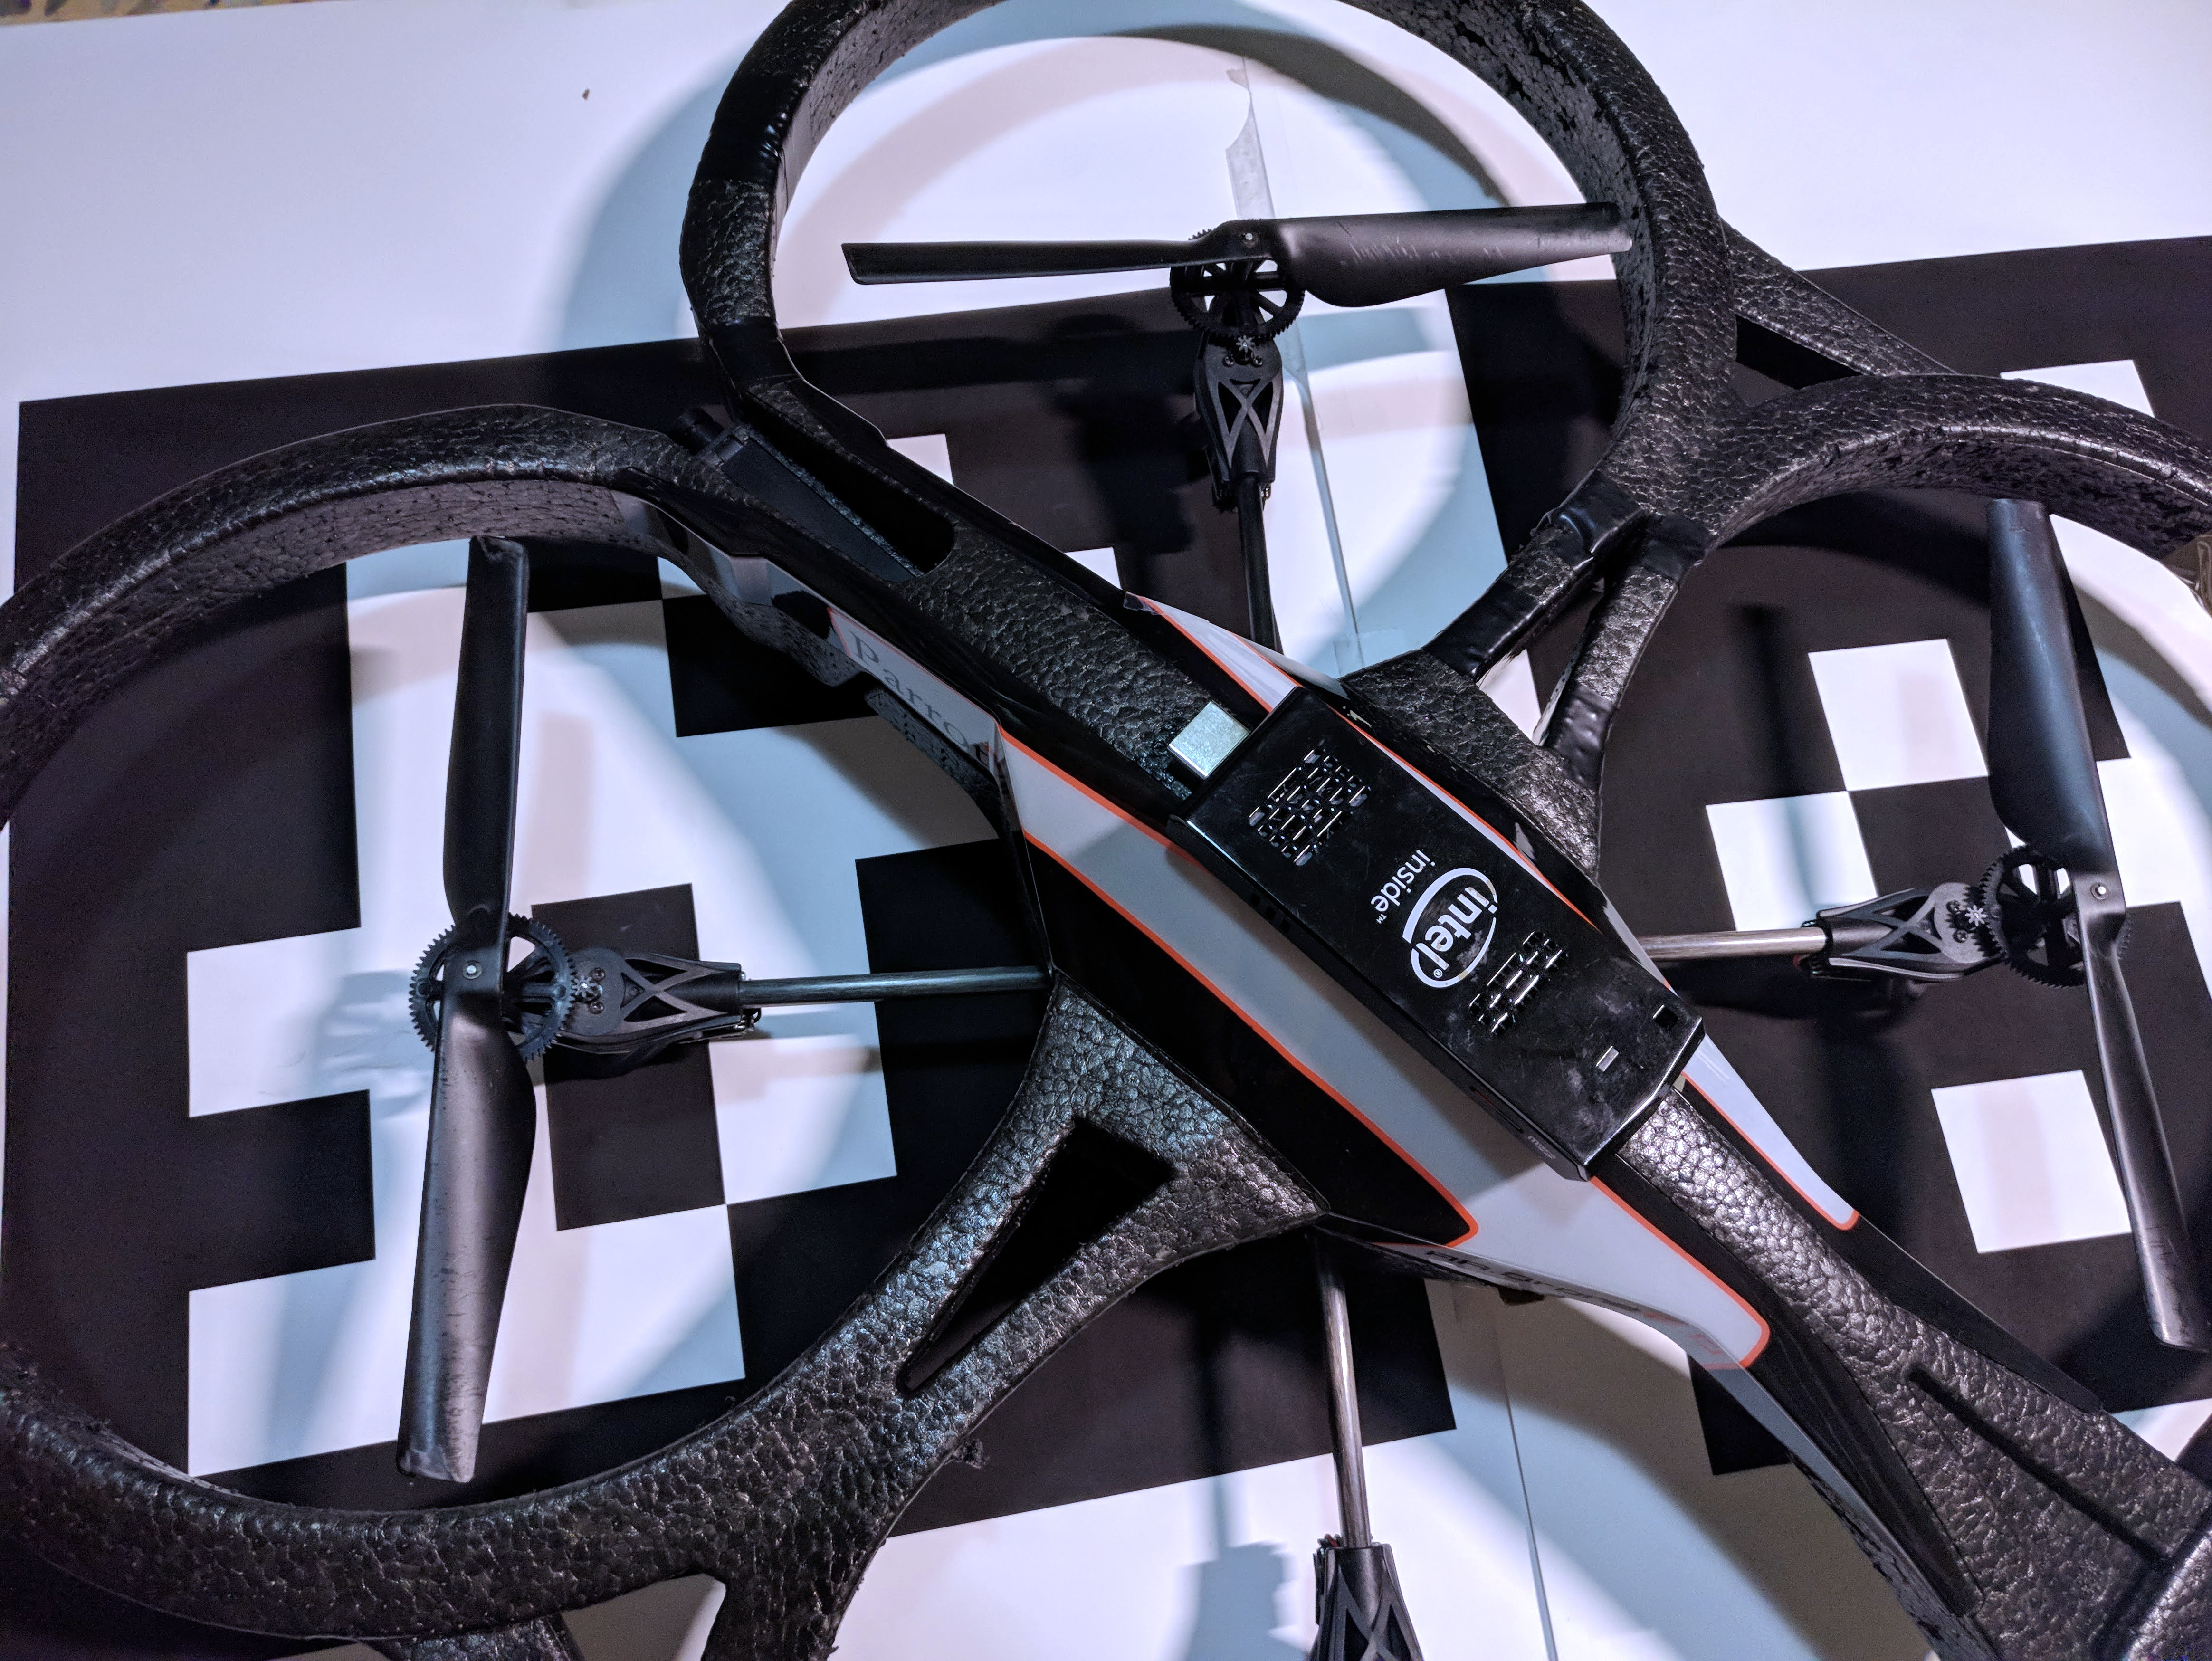
\includegraphics[width=1\textwidth]{imag/ics_drone_calibrated.jpg}
		\caption{Intel Compute Stick acoplado en Ar.Drone 2.}
		\label{fig:intelAcoplado}	
	\end{center}
\end{figure}

Además de haber instalado Ubuntu en la versión 16.04, junto a todas las dependencias y bibliotecas necesarias para correr la aplicación, se ha configurado el asistente de la red Wi-Fi para que se conecte de manera automática cuando detecte que la red que genera el drone. Se configuró la IP como estática para poder acceder de forma remota y conocer la dirección exacta de nuestra unidad de computación externa. 

Por último, se ha configurado un servidor utilizando la tecnología OpenSSH de manera que se inicie durante el lanzamientos del Sistema Operativo y que escuche en el puerto 22998. Esto  aportará una capa de seguridad, actualmente no existente además de habilitar el acceso remoto.

\subsection{Teleoperación con miniordenador a bordo}

El primer paso sería realizar una prueba teleoperando la infraestructura \ref{fig:intelAcoplado} desde nuestra herramienta uav\_viewer\_py modificado para observar cualquier cambio en el comportamiento. Lamentablemente el drone se volvía completamente inestable: desde el despegue, pasando por movimientos erráticos y no controlados, independientemente del envío de órdenes o no al drone. La limitación de potencia por parte del drone es la culpable, por lo que la única solución posible es la de realizar las pruebas sin montar a bordo el co-procesador.

\subsection{Retardo detectado en uav\_viewer\_py}

La ejecución de las pruebas unitarias reflejaba un comportamiento muy oscilante debido posiblemente a algún tipo de retardo, por lo que las primeras sospechas apuntaban a la diferencia de rendimiento entre el Intel Compute Stick y el ordenador externo de la sección anterior. Se caracterizó este retardo, mostrando valores de hasta más de un segundo en algunas de las iteraciones de los estados. Para descartar posibles problemas de rendimiento, se analizó el periodo de ejecución del estado, el consumo de recursos como el procesador, la memoria RAM y el ancho de banda utilizado. Sin embargo, los resultados de estas pruebas mostraban una frecuencia mínima de 20 Hz por ejecución, chocando con los valores previamente obtenidos.

Una investigación mas profunda llevó a la conclusión de que la herramienta \texttt{uav\_viewer\_py} que se utilizó para obtener las imágenes del drone en remoto, provocaba una saturación en el canal Wi-Fi, por lo que la solución se basó en la omisión de esta aplicación durante las pruebas con el Intel Compute Stick.



\subsection{Ejecución típica con el miniordenador en tierra}

Para iniciar la aplicación, necesitaremos acceder remotamente mediante el siguiente comando: 

\begin{lstlisting}[backgroundcolor=\color{gray!15}]
ssh 192.168.1.3 -p 22988
\end{lstlisting}

Una vez dentro, lanzaremos la aplicación de manera que la ejecución se realice en el \textit{Intel Compute Stick}.

Para prevenir cualquier accidente, se ha desarrollado un programa muy sencillo, cuya única misión es la de enviar la señal de aterrizaje al drone. Este comando evita la ejecución de futuras órdenes y asegura que el aterrizaje se realizará en el menor tiempo posible.

Se pudieron ejecutar sin problemas las pruebas unitarias, dando paso a la realización de la última prueba global o ensayo general. Este fue gratamente satisfactorio, a pesar de presentar un comportamiento ligeramente inferior en cuanto a precisión y agilidad comparado con las pruebas de la fase anterior, oscilando en mayor medida.
